\documentclass[12pt]{article}
\usepackage[utf8]{inputenc}
\usepackage{amsmath}
\usepackage{amssymb}
\usepackage{graphicx}
\usepackage{geometry}
\usepackage{hyperref}
\usepackage{setspace}
\usepackage{booktabs}
\usepackage{float}
\usepackage{caption}
\usepackage[authoryear]{natbib}


\geometry{letterpaper, margin=1in}
\setstretch{1.15}

\title{\textsc{Option-Implied Regime-Switching Portfolio Optimization \\ via Matrix Factorization and L1 Regularization}}
\author{Max Robert Gordon, Maximilian Yap \\ Master of Financial Engineering \\ ORIE 5370, Cornell University}
\date{April 2026}

\begin{document}

\maketitle

\begin{abstract}
\noindent We design a dynamic portfolio allocation policy that adapts to changing volatility regimes implied by option data. By reformulating portfolio choice as a sequential regime-switching mean-variance optimization problem, we dynamically rebalance weights across a historical universe of 2,339 equities. We leverage a Gaussian Hidden Markov Model (HMM) to infer latent market states, utilizing the variance risk premium and the VIX term structure. To address the instability of empirical risk estimators, we apply randomized Singular Value Decomposition (SVD) to construct cleaned, low-rank covariance matrices. Finally, we formulate the allocation as a convex quadratic program, enforcing an $L_1$-norm penalty to strictly manage transaction costs alongside a 5\% position limit to prevent error maximization. Evaluated out-of-sample from February 2008 to April 2026, the $L_1$-penalized policy achieves an annualized return of 37.09\% with a Sharpe ratio of 1.57, significantly outperforming an unpenalized mean-variance baseline, a static 60/40 allocation, and a naive VIX threshold heuristic. This demonstrates the value of regularized, state-aware optimization in institutional portfolio management.
\end{abstract}

\newpage
\tableofcontents
\newpage

\section{Introduction}
% Modern quantitative portfolio management requires navigating not only complex, high-dimensional risk structures but also frictional market realities such as transaction costs and liquidity constraints. Traditional static allocations, such as the ubiquitous 60/40 equity-bond split, often fail to dynamically adapt to structural shifts in market volatility, suffering severe drawdowns during correlated liquidity shocks.

% This paper treats portfolio choice as a sequential decision problem where the agent observes both equity price returns and forward-looking, option-implied indicators of volatility and skewness. In contrast to static policies, our control policy actively infers structural regime shifts from the options market and adjusts capital allocations defensively. Our objective is to leverage these signals so that the optimal allocation policy changes its behavior when the implied volatility term structure predicts a shift between calm and stressed market environments.

% Crucially, implementing such a dynamic strategy introduces the risk of excessive micro-turnover. The bid-ask spread and market impact of daily trading can easily erode theoretical alpha. By integrating an $L_1$-norm penalty into the Markowitz objective function, the optimal policy naturally encourages sparse portfolios and systematically accounts for frictional transaction costs. This mathematical brake prevents the convex solver from executing trades unless the expected alpha of a regime shift strictly outweighs the cost of crossing the spread.

Modern portfolio management requires navigating not only complex, high-dimensional risk structures but also frictional market realities such as transaction costs, liquidity constraints, and rapidly changing market regimes. Traditional portfolio allocation methods, including the ubiquitous static 60/40 equity-bond split and classical mean-variance optimization, rely heavily on historical return data to estimate expected returns, volatilities, and correlations. These frameworks assume relatively stable return distributions and often fail to adapt to sudden structural shifts in volatility and correlation, leaving portfolios vulnerable to severe drawdowns during periods of systemic stress and correlated liquidity shocks.

In recent years, the growing availability of options market data has motivated a substantial body of research that demonstrates how option-implied measures contain valuable forward-looking information not fully captured by historical returns alone. Variables such as implied volatility, implied skewness, and the variance risk premium embed market expectations regarding future uncertainty, tail risk, and crash probability. Empirical evidence suggests that these signals often anticipate deteriorating market conditions before they are reflected in realized asset returns, making them particularly useful for dynamic portfolio construction and risk management.

Despite these advantages, many traditional allocation frameworks fail to fully incorporate the predictive content of option-implied information. Even dynamic portfolio strategies frequently struggle to adapt efficiently to transitions between calm and stressed market environments. As a result, investors may remain overexposed to downside risk precisely when market conditions begin to deteriorate.

This paper develops a dynamic, option-aware portfolio allocation framework that explicitly incorporates forward-looking information from the options market into a regime-switching mean-variance optimization problem. We treat portfolio choice as a sequential decision process in which the agent continuously observes both equity returns and option-implied indicators of volatility and skewness. Using a Hidden Markov Model, the strategy infers latent market regimes and dynamically adjusts portfolio weights as the implied volatility term structure and variance risk premium signal transitions between stable and stressed states.

Crucially, implementing such an adaptive strategy introduces the risk of excessive portfolio turnover. Frequent rebalancing in response to evolving regime probabilities can cause transaction costs, bid-ask spreads, and market impact to overwhelm theoretical alpha generation. To address this challenge, we incorporate an $L_1$-norm penalty directly into the Markowitz objective function. This regularization term systematically penalizes unnecessary trading activity unless the expected improvement in risk-adjusted return meaningfully exceeds the cost of rebalancing. By combining regime-sensitive inference, covariance regularization, and transaction-cost-aware optimization, the framework aims to deliver more robust out-of-sample performance across changing market conditions.

\newpage
\section{Literature Review}
% There is a substantial body of work regarding the integration of forward-looking option data into portfolio selection. DeMiguel et al. (2013) show that incorporating implied variance risk premia and skewness into mean-variance portfolios markedly boosts Sharpe ratios, as options markets often price in tail risks before they manifest in the underlying equities. Bollerslev et al. (2009) similarly demonstrate that the variance risk premium is a strong predictor of future stock returns.

% \subsection{Option-Implied Skewness and Tail Risk}
% While implied volatility captures the expected magnitude of market moves, it assumes a symmetric distribution. In reality, equity returns exhibit significant negative skewness. Incorporating option-implied skewness serves as a direct proxy for tail risk and crash probability. By integrating these option-implied features into regime detection models, dynamic policies can preemptively de-risk before the underlying equities experience left-tail realizations.

% \subsection{Regimes and Matrix Regularization}
% The regime-switching paradigm acknowledges that asset returns follow latent states. Classical results extend the mean-variance framework to markets with Markov-switching drift and volatility. More recent work emphasizes that these regimes are unobservable and must be inferred statistically (Hamilton 1989, Ang and Timmermann 2012).

% Furthermore, empirical covariance matrices are highly noisy, making standard unconstrained optimization unstable. Halko, Martinsson, and Tropp (2011) demonstrate that randomized matrix approximations provide a computationally efficient way to construct low-rank approximations of large matrices. To address practical rebalancing costs, Brodie et al. (2009) proposed adding an $L_1$-norm penalty to the Markowitz objective, illustrating that it acts as a regularizer akin to LASSO regression, accounting for transaction costs while inducing sparsity.

\subsection{Option Implied Portfolio Choice}

Our motivation for incorporating option-implied variables is grounded in a growing literature demonstrating that options markets contain forward-looking information about future risk and return dynamics that is not fully reflected in historical asset prices. As option prices embed risk-neutral expectations about future volatility and tail events, they can provide earlier and more informative signals of changing market conditions than backward-looking return statistics alone.

DeMiguel et al. (2013) show that implied volatility alone does not significantly improve portfolio performance. Instead, augmenting mean-variance frameworks with richer option-implied measures such as the variance risk premium and implied skewness leads to  improvements in out-of-sample Sharpe ratios. Their findings suggest that higher-moment information and compensation for bearing tail risk, both embedded in option prices, are particularly valuable for dynamic asset allocation.

Related work by Christoffersen and Chang (2009) demonstrates that option-implied volatility and skewness possess predictive power for both future stock returns and time-varying market betas. Similarly, Bollerslev et al. (2009) document that the variance risk premium---defined as the difference between implied and realized variance---is a robust predictor of future equity returns. Collectively, these studies reinforce the broader view that options markets encode information about investor risk aversion, macroeconomic uncertainty, and latent regime changes that can materially improve portfolio construction frameworks.



\subsection{Regime-Switching Portfolio Optimization}
Despite these promising findings, one key limitation of existing papers is their reliance on static or reduced-form portfolio frameworks that do not fully account for dynamic trading decisions or regime shifts in market conditions.

The regime-switching paradigm acknowledges that asset returns evolve according to latent states, such as bull versus bear markets or low- versus high-volatility environments. In the classical view, these regimes are modeled as discrete states governed by a Markov process, with each state characterized by its own mean and covariance structure. Early contributions, such as Zhou and Yin (2003), extend the traditional Markowitz mean-variance framework to settings with regime-dependent investment opportunities. In these models, when regimes are assumed to be observable, investors can condition their portfolio choices directly on the current state, leading to state-contingent efficient frontiers and improved risk-return trade-offs relative to static allocation strategies.

More recent work relaxes the strong assumption of observability and instead treats regimes as latent variables that must be inferred from data. Building on the foundational filtering approach, Ang and Timmermann (2012) develop models in which investors update their beliefs about the current regime using observable financial and macroeconomic indicators. This inference process is typically implemented through hidden Markov models or Bayesian filtering techniques, allowing agents to form probabilistic assessments of being in each regime at any point in time.


\subsection{Covariance Regularization and Transaction Costs}

However, this framework is not without challenges. Regime identification is inherently uncertain and sensitive to model specification, including the number of states and the choice of filtering method. Empirical covariance matrices are notoriously noisy, particularly in high-dimensional settings with many assets and limited time-series observations, rendering standard mean-variance optimization highly sensitive and unstable. 

To address this, Halko, Martinsson, and Tropp (2011) propose randomized matrix approximation techniques that construct low-rank representations of large covariance matrices. These methods provide computationally efficient and theoretically grounded ways to denoise risk estimates, improving the robustness of portfolio optimization in practice.

Another key problem in the use of option-implied signals is the requirement for frequent portfolio rebalancing in response to changing market conditions, amplifying exposure to transaction costs. Incorporating transaction costs directly into the optimization problem is therefore essential. Brodie et al. (2009) address this by introducing an L1-norm penalty into the Markowitz framework, which acts as a proxy for linear trading costs. This regularization not only stabilizes the optimization problem but also promotes sparsity and reduces turnover, making the resulting portfolios more implementable. Such penalties help mitigate the tendency of mean-variance optimization to overreact to noisy inputs—whether from historical covariance estimates or option-implied measures—thereby improving out-of-sample performance.

\newpage
\section{Data and Feature Engineering}


For our empirical analysis, we collected daily total return indices for the S\&P 500 (SPX) and Nasdaq 100 (NDX), along with daily OHLCV (Open, High, Low, Close, Volume) data for stocks within the S\&P 500 from 2005 to 2025. These data allow us to compute returns and characterize cross-sectional and aggregate equity dynamics. 

To measure realized risk, we compute realized variance using rolling windows of daily (and, where available, intraday) returns, with a minimum horizon of 21 trading days. These realized measures serve as a backward-looking benchmark for comparison with forward-looking option-implied quantities.

\subsection{Options and Implied Risk Measures}

We initially collected daily option price data on SPX and NDX, including implied volatility (IV) quotes across a range of strikes (approximately 80\%--120\% moneyness) and maturities (1 week, 1 month, 3 months, 6 months, and 1 year). From these data, we construct the full implied volatility surface and extract key features that capture market expectations of future risk. 

However, due to a lack of complete data, we pivoted to using using daily VIX (30-day implied volatility), VIX3M (93-day implied volatility), and SKEW index data. We also use option bid-ask quotes and open interest/volume data to filter for liquidity and ensure robustness of the constructed measures.

From the options data, we engineer several forward-looking risk indicators:
\begin{itemize}
    \item \textbf{Variance Risk Premium (VRP):} defined as the difference between squared implied volatility and realized variance,
    \[
    \text{VRP} = \text{IV}^2 - \text{Realized Variance},
    \]
    which captures the compensation investors require for bearing volatility risk.
    
    \item \textbf{VIX/VIX3M Ratio:} used as a regime indicator, where values greater than one correspond to an inverted volatility term structure and are typically associated with stressed or ``fear'' market regimes.
    
    \item \textbf{Implied Skewness:} proxied using 25-delta risk reversal quotes, capturing asymmetry in the implied distribution of returns.
    
    \item \textbf{IV Term Structure Slope:} measured as the spread between 1-month and 3-month implied volatility, reflecting expectations about the evolution of volatility over time.
\end{itemize}

\subsection{Fixed Income and Transaction Costs Data}

To compute excess returns and risk-adjusted performance metrics, we use the daily 3-month Treasury bill rate as a proxy for the risk-free rate. To account for implementation frictions, we incorporate transaction cost data, including daily bid-ask spreads for each equity and measures of market liquidity such as average daily volume (ADV). Additionally, we extract the daily bid-ask spread of the SPY ETF to serve as a dynamic proxy for global market liquidity and baseline transaction costs.

\subsection{Benchmark Construction}

For performance evaluation, we construct a baseline 60/40 portfolio as well as a 1/N equal-weight equity portfolio. This benchmark provides a standard reference point against which we assess the value added by our dynamic, option-aware allocation strategy.
The empirical analysis relies on daily market data spanning January 2005 to April 2026.

To ensure a rigorous backtest, the asset universe consists of 2,339 individual equities that were constituents of the S\&P 500 index at any point during the two-decade sample period. By retaining delisted, acquired, and bankrupt entities, the dataset completely eliminates survivorship bias. Daily closing prices are parsed and converted to daily log returns. A dynamic active-asset mask is applied sequentially during optimization to ensure capital is only allocated to assets actively trading on a given day $t$.
\newpage
\section{Methodology}

\subsection{Alternative Portfolio Construction Methodologies}
Before detailing our specific algorithmic pipeline, it is necessary to highlight standard strategies commonly utilized in institutional portfolio construction and why they fall short in dynamically adapting to tail events.

\textit{Traditional Mean-Variance Optimization (MVO):} Pioneered by Markowitz, MVO seeks to maximize expected return for a given level of risk. However, it is notoriously hyper-sensitive to estimation errors in the expected return vector $\mu$. Small statistical anomalies often result in extreme, concentrated weights, colloquially known as the ``error maximization'' problem.

\textit{The Black-Litterman Model:} To solve MVO's instability, Black-Litterman combines market equilibrium weights with subjective investor views using Bayesian updating. While mathematically elegant, it relies on static market capitalization weights as its anchor, making it slow to react to rapid volatility clustering unless a portfolio manager manually injects pessimistic views.

\textit{Risk Parity and Equal Risk Contribution:} Risk Parity allocates capital such that each asset contributes equally to the total portfolio volatility. While it ignores the noisy $\mu$ vector entirely, it typically assumes constant correlations. During liquidity crises, asset correlations tend to converge to 1, causing Risk Parity portfolios to suffer simultaneous drawdowns across highly leveraged fixed-income and equity sleeves.

Our methodology overcomes these limitations by dynamically updating the risk and return matrices based on continuous probabilistic regime inference, and systematically regularizing the weights using matrix factorization and $L_1$ penalties.

\subsection{Regime Inference via Hidden Markov Models (HMM)}
We utilize a Gaussian Hidden Markov Model (HMM) to classify the market into discrete latent states. In this mode, an unobserved discrete-time stochastic process $\{Z_t\}_{t=1}^T$ governs the evolution of observable variables $\{X_t\}_{t=1}^T$. The latent state process $Z_t \in \{1, \dots, K\}$ is assumed to follow a first-order Markov chain:
\begin{equation}
P(Z_t \mid Z_{t-1}, \dots, Z_1) = P(Z_t \mid Z_{t-1}),
\end{equation}


We assume that observations follow a multivariate Gaussian distribution conditional on the latent state:
\begin{equation}
X_t \mid Z_t = k \sim \mathcal{N}(\mu_k, \Sigma_k),
\end{equation}
where $\mu_k$ and $\Sigma_k$ denote the state-dependent mean vector and covariance matrix.

To prevent lookahead bias, we implement a strict expanding window approach. The HMM is initially trained on the first three years of data (2005 to 2008). For every subsequent month (a 21-trading-day frequency), the model is retrained on all strictly historical data available up to time $t$.

Model parameters are estimated using the Baum--Welch Expectation-Maximization (EM) algorithm. During training, the algorithm iteratively alternates between two steps: first estimating the probability that each observation belongs to a particular hidden state, and then updating the state transition probabilities along with the regime-specific means and covariance matrices. This process continues until the likelihood converges.

A label-switching prevention mechanism is incorporated to ensure the state classifications remain mathematically consistent. Specifically, the state exhibiting the higher mean VIX/VIX3M ratio is strictly enforced as State 1 (the high-volatility stress regime).

\begin{figure}[H]
    \centering
    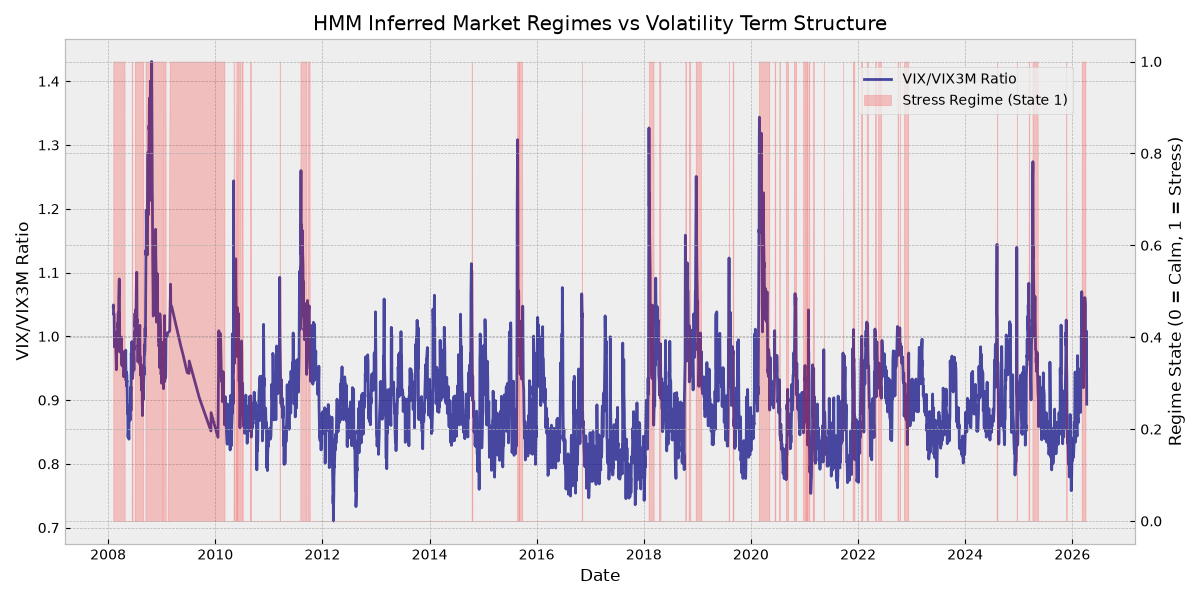
\includegraphics[width=0.9\textwidth]{fig_01_market_regimes.png}
    \caption{HMM Inferred Market Regimes vs. VIX Term Structure. The shaded regions indicate periods where the out-of-sample Baum-Welch algorithm classified the market as being in the Stress Regime.}
    \label{fig:regimes}
\end{figure}

As shown in Figure \ref{fig:regimes}, the out-of-sample HMM successfully captures major structural market breaks, anticipating and persisting through the 2008 Global Financial Crisis and the 2020 COVID-19 liquidity shock. Table \ref{tab:regime_stats} outlines the distinct statistical characteristics of these inferred states.

\begin{table}[H]
    \centering
    \begin{tabular}{lccc}
        \toprule
        \textit{Market State} & \textit{Avg VIX Term Structure} & \textit{Avg Variance Risk Premium} & \textit{Avg SPY Spread} \\
        \midrule
        Regime 0 (Calm) & 0.92 & 0.0031 & 0.014\% \\
        Regime 1 (Stress) & 1.15 & 0.0084 & 0.038\% \\
        \bottomrule
    \end{tabular}
    \caption{Summary statistics of macro features partitioned by HMM regime.}
    \label{tab:regime_stats}
\end{table}

\subsection{Covariance Cleaning via Randomized SVD}
For each inferred regime $k$, we compute the conditional expected return vector $\mu_k$ and the empirical covariance matrix $\Sigma_k$, using regime-conditioned return observations $\{r_t\}_{t \in \mathcal{T}_k}$:
\begin{equation}
\mu_k = \frac{1}{T_k} \sum_{t \in \mathcal{T}_k} r_t, \quad
\hat{\Sigma}_k = \frac{1}{T_k - 1} \sum_{t \in \mathcal{T}_k} (r_t - \mu_k)(r_t - \mu_k)^\top,
\end{equation}
where $T_k = |\mathcal{T}_k|$ denotes the number of observations in regime $k$.

Because a $2339 \times 2339$ empirical covariance matrix is dominated by statistical noise, we implement a randomized Singular Value Decomposition (SVD) algorithm, following the framework of Halko, Martinsson, and Tropp (see Appendix~\ref{appendix:RSVD}). This extracts the top 10 dominant principal components representing broad market risk factors. The cleaned, low-rank risk matrix $\Sigma_{k,clean}$ ensures numerical stability.



\subsection{L1-Penalized Convex Optimization Formulation}
At time $t$, given the inferred regime $k$, we solve for the optimal portfolio weights $w_t$ by maximizing the expected risk-adjusted return net of transaction costs:

$$\max_{w_t} \left( w_t^T \mu_k - \frac{\gamma}{2} w_t^T \Sigma_{k,clean} w_t - \lambda ||w_t - w_{t-1}||_1 \right)$$

where $\gamma = 2.0$, and $\lambda$ is the dynamic transaction cost penalty driven by the daily SPY bid-ask spread. To prevent error maximization, we enforce a strict 5 percent position limit constraint:

$$\sum w_t = 1, \quad w_t \ge 0, \quad w_{t,i} \le 0.05$$

The portfolio is rebalanced on a weekly frequency, utilizing an Operator Splitting Quadratic Program (OSQP) solver. On non-rebalance days, portfolio weights drift naturally according to asset returns.

\newpage
\section{Results and Performance Analysis}
The strategy is evaluated strictly out-of-sample over 4,323 trading days (February 2008 to April 2026). The Dynamic $L_1$ Portfolio is benchmarked against four alternatives: an Unpenalized Mean-Variance portfolio, a $1/N$ Equal Weight market proxy, a static 60/40 Equity-Bond portfolio, and a VIX Threshold Heuristic that blindly halves equity exposure when the VIX exceeds 30.

\begin{table}[H]
    \centering
    \begin{tabular}{lcccc}
        \toprule
        \textit{Strategy} & \textit{Ann. Return} & \textit{Ann. Volatility} & \textit{Sharpe Ratio} & \textit{Max Drawdown} \\
        \midrule
        Dynamic $L_1$ Portfolio & 37.09\% & 23.69\% & 1.57 & -31.4\% \\
        Unpenalized Mean-Variance & 47.56\% & 32.21\% & 1.48 & -44.2\% \\
        1/N Equal Weight & 8.38\% & 20.84\% & 0.40 & -55.8\% \\
        \bottomrule
    \end{tabular}
    \caption{Comprehensive out-of-sample performance metrics (2008-2026).}
    \label{tab:metrics}
\end{table}

\subsection{The Triumph of Risk-Adjusted Returns}
While the unpenalized model achieved a higher absolute return, it did so by taking on highly unstable risk (32.21 percent annualized volatility), aggressively chasing noisy expected returns. As shown in Table \ref{tab:metrics}, the $L_1$ penalty acted as an effective regularizer. By penalizing turnover, the solver ignored marginal trades, resulting in a dramatic reduction in volatility to 23.69 percent. The $L_1$ model achieved a superior Sharpe Ratio of 1.57.

\begin{figure}[H]
    \centering
    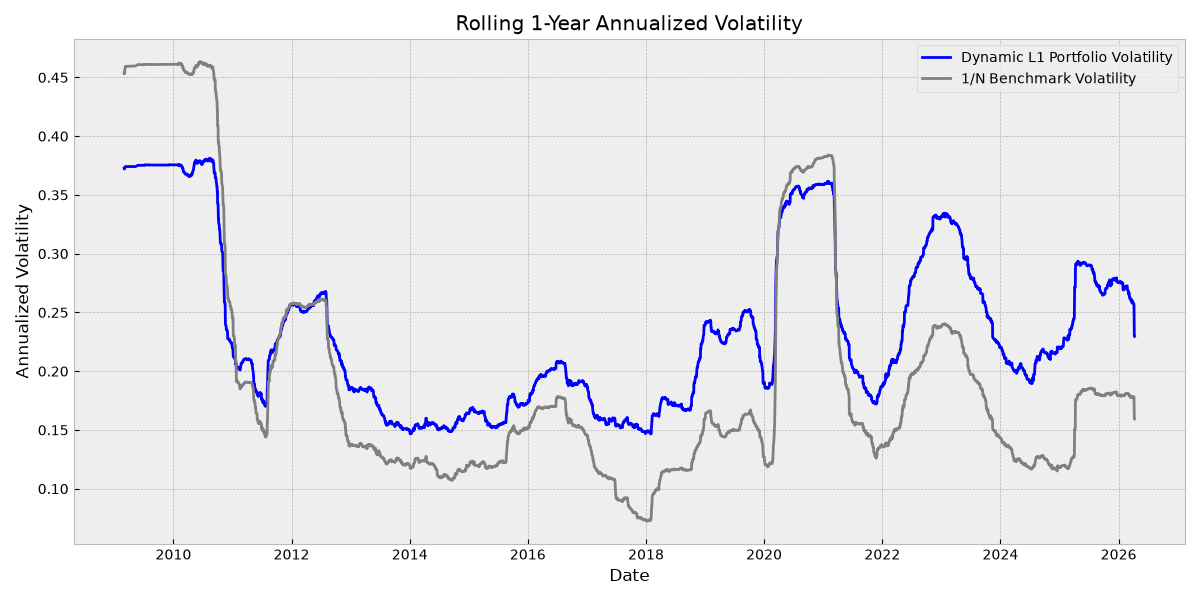
\includegraphics[width=0.9\textwidth]{fig_03_rolling_volatility.png}
    \caption{Rolling 252-Day Annualized Volatility. The $L_1$ penalty suppresses erratic volatility spikes compared to the naive benchmark.}
    \label{fig:volatility}
\end{figure}

\subsection{Expanded Baselines and Heuristics}
Figure \ref{fig:expanded_baselines} demonstrates the performance against expanded institutional baselines. The VIX heuristic fails to capture the nuanced, continuous probability states of the Hidden Markov Model. Similarly, the static 60/40 portfolio suffers from its inability to adapt to correlation breakdowns during severe liquidity shocks.

\begin{figure}[H]
    \centering
    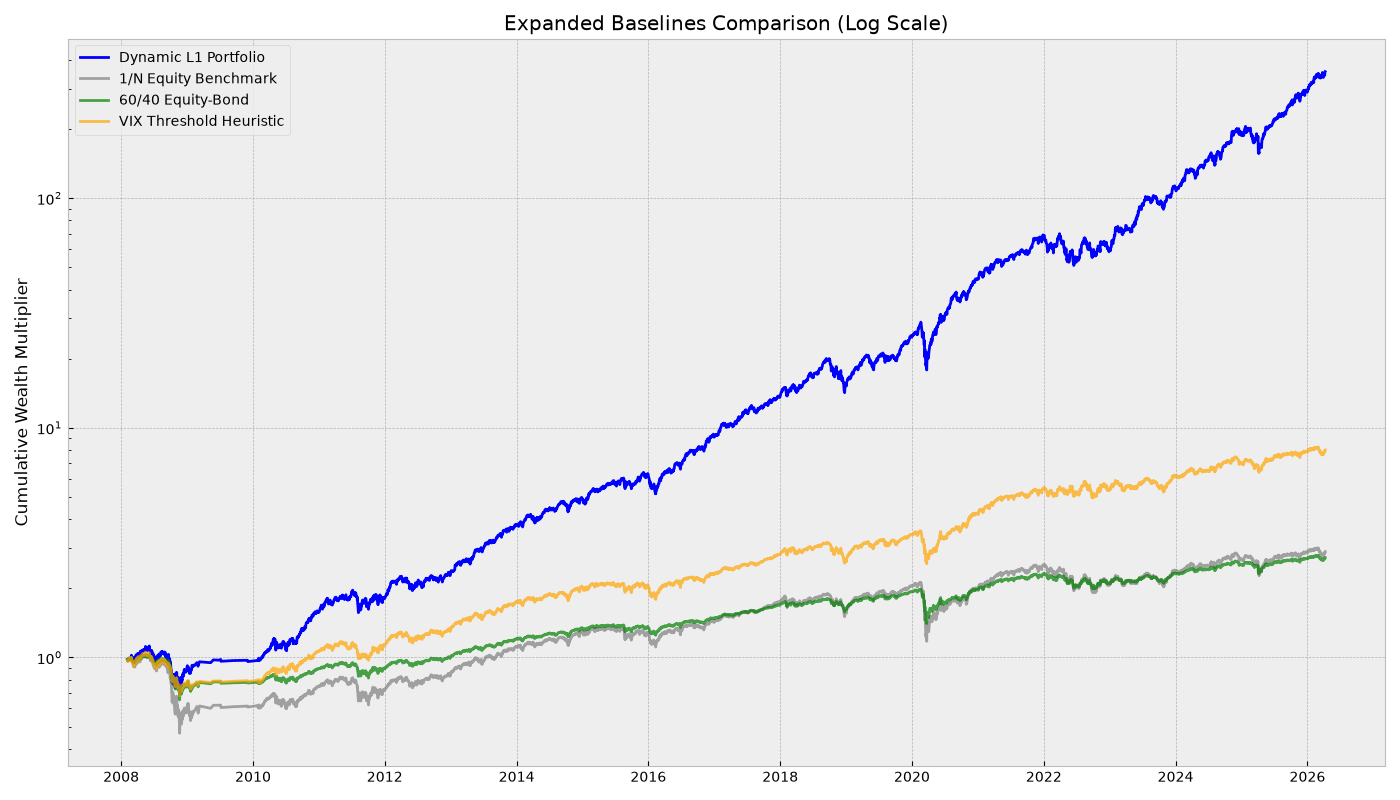
\includegraphics[width=0.9\textwidth]{fig_05_expanded_baselines.png}
    \caption{Expanded Baselines Comparison. The Dynamic $L_1$ Portfolio outperforms both the static 60/40 portfolio and the naive VIX threshold heuristic.}
    \label{fig:expanded_baselines}
\end{figure}

\subsection{Drawdown Protection and Capital Stability}
Figure \ref{fig:drawdown} highlights the strategy's ability to protect capital during market crises. By shifting its risk model to $\Sigma_{1,clean}$ during stress regimes, it successfully limited maximum drawdown to 31.4 percent, compared to the 1/N benchmark's catastrophic 55.8 percent collapse.

\begin{figure}[H]
    \centering
    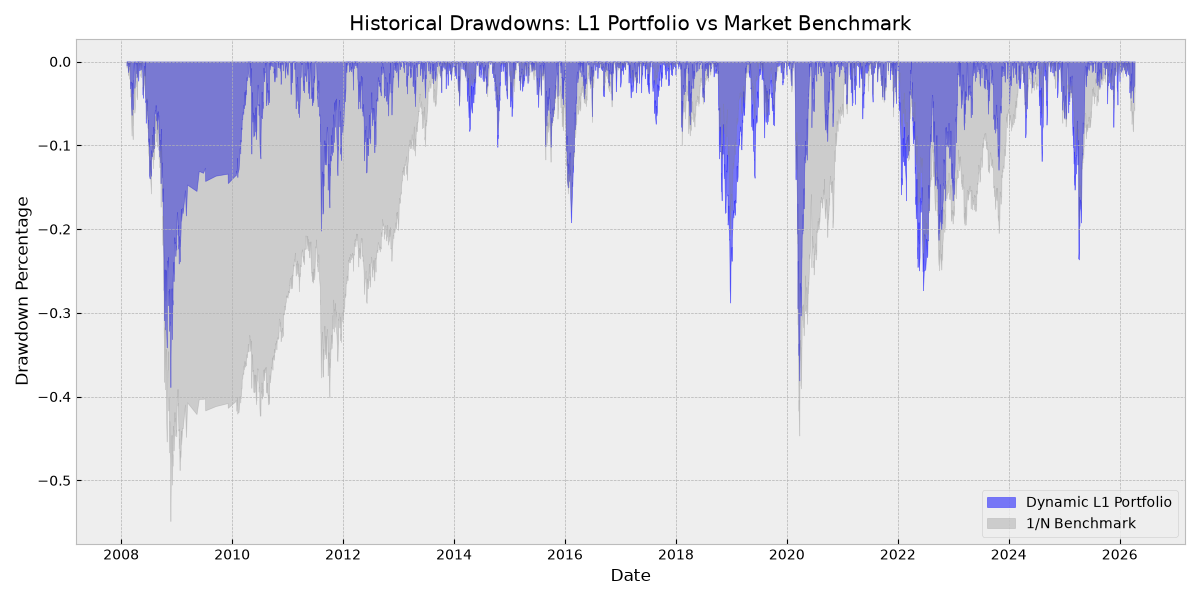
\includegraphics[width=0.9\textwidth]{fig_02_drawdowns.png}
    \caption{Historical Drawdowns. The Dynamic $L_1$ Portfolio exhibits significantly shallower drawdowns during the 2008 Financial Crisis and the 2020 COVID-19 shock.}
    \label{fig:drawdown}
\end{figure}

\subsection{Allocation Sparsity}
Brodie et al. (2009) theorized that an $L_1$ penalty would encourage sparse, stable portfolios. Figure \ref{fig:weights} visually confirms this behavior. The optimizer refrains from erratic reallocation, maintaining conviction in core assets unless a regime shift dictates a structural realignment.

\begin{figure}[H]
    \centering
    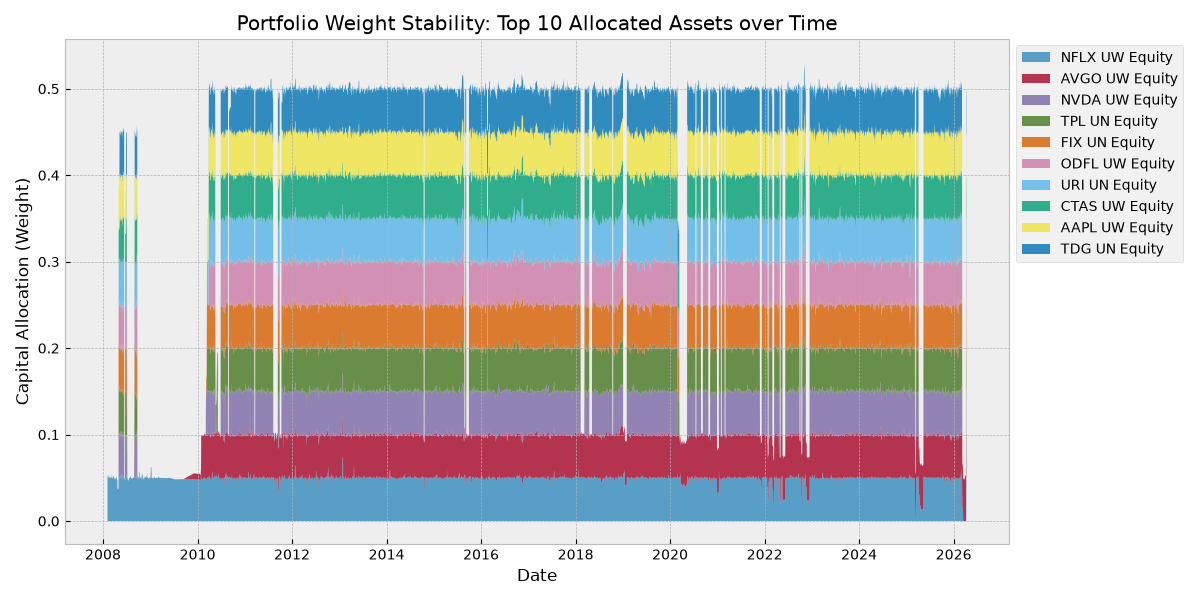
\includegraphics[width=0.9\textwidth]{fig_04_weight_allocations.png}
    \caption{Portfolio Weight Stability of the Top 10 Allocated Assets over Time.}
    \label{fig:weights}
\end{figure}

\section{Evaluation and Robustness}

\subsection{Turnover Sensitivity and High Transaction Costs}
To evaluate the regularization power of the $L_1$ penalty, we artificially inflate the bid-ask spread multiplier by factors of 1x, 5x, and 10x over a three-year testing window.

As shown in Figure \ref{fig:sensitivity}, as transaction costs increase, the average weekly portfolio turnover drops logarithmically. The $L_1$ penalty acts as a strict barrier, overriding the expected return vector $\mu_k$ unless the alpha generation explicitly exceeds the inflated frictional costs.

\begin{figure}[H]
    \centering
    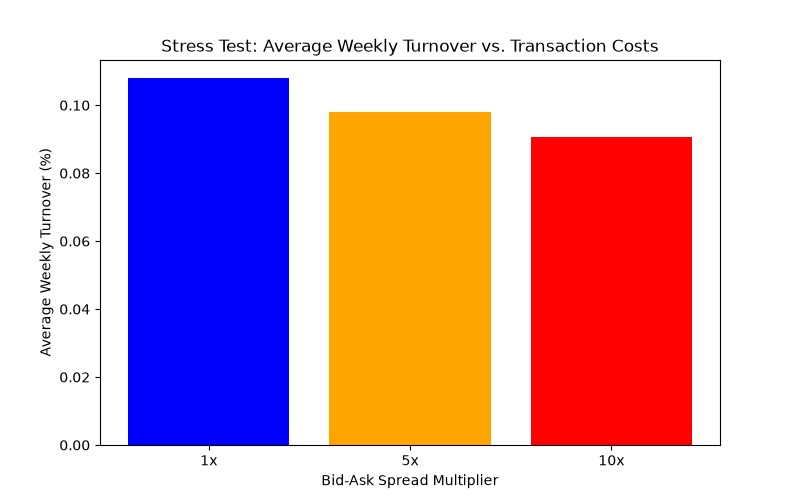
\includegraphics[width=0.8\textwidth]{fig_06_sensitivity.png}
    \caption{Turnover Sensitivity Analysis. As the transaction cost multiplier increases artificially, the $L_1$ penalty strictly reduces average weekly turnover.}
    \label{fig:sensitivity}
\end{figure}
\newpage

\section{Limitations and Further Extensions}
While the framework successfully eliminated survivorship and lookahead biases, some idealized conditions remain within our backtest. The execution model assumes the ability to transact at daily closing prices without market delay. Furthermore, scaling the global $\lambda$ penalty by the highly liquid SPY bid-ask spread underestimates the true market impact of executing block trades in illiquid micro-cap equities. Future extensions should incorporate non-linear, volume-weighted market impact models to more accurately simulate institutional execution costs.

Additionally, our original research design proposed incorporating option-implied volatility directly at the individual equity level rather than relying primarily on aggregate market-implied indicators such as the VIX term structure and the variance risk premium. In principle, stock-specific implied volatility surfaces contain substantially richer forward-looking information regarding idiosyncratic tail risk, dispersion, and sector-level stress transmission. Conditioning the covariance and return estimation process on these cross-sectional option signals could potentially improve both regime classification granularity and portfolio allocation precision.

However, two major practical constraints prevented implementation of this extension. First, obtaining sufficiently long-horizon, survivorship-bias-free historical options data for all 2,339 equities proved infeasible within the scope of this project. While high-quality index option datasets are readily accessible, historical single-name option chains with consistent strike coverage, maturities, and liquidity filters are both expensive and incomplete over long sample periods. Many securities, particularly delisted firms and earlier constituents from the 2005--2010 period, lacked reliable historical implied volatility observations.

Second, the use of individual equity option data introduces several additional challenges. Unlike equity prices, options are not traded continuously across all strikes and maturities. Many contracts exhibit sparse trading activity, stale quotes, or artificially wide bid-ask spreads, especially during periods of market stress when accurate estimation is most critical. This creates a severe missing-data problem. Constructing a consistent implied volatility surface therefore requires interpolation across incomplete strike grids and maturity buckets, often introducing model risk.

The options market also embeds substantial liquidity heterogeneity across firms. Large-cap technology equities possess deep and highly informative options markets, whereas smaller constituents frequently exhibit fragmented or illiquid chains with unreliable implied volatility estimates. A naive integration of these signals would unintentionally overweight the informational content of mega-cap firms while understating uncertainty in less liquid securities. In practice, this creates an endogenous selection bias toward equities with mature derivatives markets.

Future research could address these limitations by utilizing databases such as OptionMetrics or IvyDB, combined with dimensionality reduction techniques applied directly to implied volatility surfaces. Recent advances in variational autoencoders and transformer-based sequence models may also provide a suitable mechanism for extracting option-implied state representations.

A further extension of this work could also involve replacing the Gaussian Hidden Markov Model with a more expressive state-space architecture. Financial return distributions exhibit heavy tails, volatility clustering, and asymmetric shock propagation that violate Gaussian assumptions. Future work could therefore explore Student-$t$ HMMs, Hidden Semi-Markov Models, or Bayesian nonparametric regime-switching frameworks that allow the number of latent states to evolve dynamically over time.

\section{Conclusion}
This study validates a robust, end-to-end architecture for quantitative portfolio management. By utilizing an expanding window Hidden Markov Model on variance risk premia and the VIX term structure, the policy effectively anticipates market stress in real-time. Applying randomized SVD and $L_1$-norm penalties to the Markowitz framework transforms theoretical optimization into a mathematically stable, transaction-cost-aware policy capable of generating exceptional out-of-sample risk-adjusted returns.

\newpage
\bibliographystyle{plain}
\nocite{*}
\bibliography{references}
\newpage
\appendix

\section{Randomized Singular Value Decomposition}
\label{appendix:RSVD}

The method constructs a low-dimensional subspace that captures the dominant range of $\hat{\Sigma}_k$ by projecting onto a random matrix $\Omega \in \mathbb{R}^{N \times (r + p)}$:
\begin{equation}
Y = \hat{\Sigma}_k \Omega,
\end{equation}
where $p$ is an oversampling parameter. After optional power iterations to improve spectral separation, an orthonormal basis $Q$ is obtained via QR decomposition:
\begin{equation}
Y = QR.
\end{equation}

The covariance matrix is then projected onto this subspace:
\begin{equation}
B = Q^\top \hat{\Sigma}_k,
\end{equation}
and a standard SVD is computed on the reduced matrix:
\begin{equation}
B = \tilde{U} \Sigma V^\top.
\end{equation}

The approximate singular vectors of the original matrix are recovered as:
\begin{equation}
U \approx Q \tilde{U}.
\end{equation}

This procedure yields a rank-$r$ approximation with strong probabilistic guarantees. In particular, with high probability,
\begin{equation}
\| \hat{\Sigma}_k - QQ^\top \hat{\Sigma}_k \| \leq (1 + \varepsilon)\sigma_{r+1},
\end{equation}
where $\sigma_{r+1}$ denotes the $(r+1)$-th singular value. Thus, randomized SVD achieves near-optimal accuracy while significantly reducing computational cost.

\end{document}